% SPDX-FileCopyrightText: Copyright (c) 2026 Nasir Ali, C-DAC Noida
% SPDX-License-Identifier: Apache-2.0
\documentclass[pdflatex,sn-basic]{sn-jnl}

\usepackage{mathrsfs}
\usepackage{graphicx}
\usepackage{multirow}
\usepackage{amsmath,amssymb,amsfonts}
\usepackage[title]{appendix}
\usepackage{xcolor}
\usepackage{textcomp}
\usepackage{booktabs}
\usepackage[utf8]{inputenc}
\usepackage{algorithm}
\usepackage{algpseudocode}
\usepackage{url}
\usepackage{hyperref}

\raggedbottom

\begin{document}

\title[An FPGA Reimplementation of a Neural Pre-Decoder]{An FPGA Reimplementation and Honest Evaluation of a Neural Pre-Decoder for Surface-Code Quantum Error Correction}

\author*[1]{\fnm{Nasir} \sur{Ali}}\email{nasirali2607@gmail.com}

\affil*[1]{\orgdiv{Embedded Systems Division}, \orgname{Centre for Development of Advanced Computing (C-DAC)}, \orgaddress{\city{Noida}, \postcode{201307}, \state{Uttar Pradesh}, \country{India}}}

\abstract{Neural pre-decoders have been proposed as a way to reduce the syndrome volume that a classical matching decoder must resolve on every round of surface-code quantum error correction, with the goal of easing the real-time latency budget imposed by qubit coherence times. This paper presents an independent, from-scratch FPGA reimplementation of that concept, targeting a Xilinx Alveo U55C: a fully convolutional 3D CNN pre-decoder trained on simulated rotated-surface-code syndromes, a quantization study (INT8, INT4, ternary) with exported fixed-point weights, a Vitis HLS kernel synthesized and placed-and-routed to a real, timing-closed bitstream, and host integration code against the real XRT API. Unlike a typical results paper, this one reports a mixed and partially negative outcome as its primary finding, because that is what the reproducible experiments show: at the code distance used for training (\(d=5\)), the trained pre-decoder's logical error rate is consistently worse than a PyMatching-only baseline across the tested noise range, and this disadvantage widens by roughly three orders of magnitude by \(d=13\), the opposite of the distance-generalization property the fully convolutional architecture is intended to provide. Independent of that result, quantization is a clean success: INT8 and ternary weights cost negligible additional logical error rate relative to FP32, while INT4 shows a consistent regression. The synthesized kernel initially exceeded the target device's on-chip memory budget by more than 11x due to a fully unrolled multiply-accumulate loop; root-causing and fixing this defect is described in detail, along with the subsequent discovery and resolution of an unclosed timing-closure violation in the first successful place-and-route attempt. The result is a real, working, timing-closed bitstream whose measured per-shot latency (13.0--15.3\,ms) remains roughly four orders of magnitude above the method's aspirational microsecond-scale target, a gap this paper quantifies rather than minimizes. Every number reported is machine-generated from a committed artifact, not hand-transcribed or estimated; all code, synthesis reports, and figures are available in a public repository.}

\keywords{Quantum error correction, surface code, neural decoder, FPGA, high-level synthesis, quantization, Alveo U55C}

\maketitle

\section{Introduction}\label{sec:introduction}

Quantum error correction (QEC) protocols based on the surface code require a classical decoder to convert a stream of syndrome measurements into a correction, ideally within the timescale set by qubit coherence and the syndrome-extraction round period \cite{fowler2012surface}. Minimum-weight perfect matching (MWPM), implemented efficiently by libraries such as PyMatching \cite{higgott2022pymatching}, is the standard decoder for surface codes and provides good accuracy, but its per-shot latency and the size of the matching graph both grow with code distance, which is a concern as devices scale toward the larger distances fault tolerance will eventually require.

A recent line of work proposes reducing this burden with a lightweight neural network, a \emph{pre-decoder}, that runs before the matching decoder and resolves a large fraction of "local" detection events on its own, shrinking the residual syndrome that MWPM has to process. NVIDIA's \texttt{Ising-Decoding} work \cite{chamberland2026fast} describes such a pre-decoder using a fully convolutional 3D CNN whose receptive field is tied to the training code distance but which, by construction, can be applied unchanged to other distances.

This paper presents an independent, from-scratch reimplementation of that concept end to end: a rotated-surface-code simulation and training data pipeline, a fully convolutional 3D CNN pre-decoder, a quantization study down to ternary weights, a synthesizable Vitis HLS kernel for a Xilinx Alveo U55C, and host integration code against the real XRT hardware API. No model weights, training code, or other artifacts from the NVIDIA repository were used; the neural network, quantization scheme, HLS microarchitecture, and latency model are original work produced for this project.

\subsection{Why report a negative result}\label{subsec:why-negative}

Most systems papers report a method that works. This one does not report that the pre-decoder improves logical error rate over the matching-only baseline; the honest, reproducible experiments in Section~\ref{sec:results} show the opposite at every tested noise rate and, worse, show the disadvantage growing rather than shrinking as code distance increases past the training distance. Two considerations motivate reporting this result rather than omitting it or reframing the paper around only the parts that succeeded. First, the negative result is itself informative: it isolates specific, nameable causes (Section~\ref{subsec:discussion-why}) rather than a vague "did not work," which is useful to anyone attempting a similar reimplementation. Second, several genuinely positive results were produced in the course of this work, most notably that INT8 and ternary quantization of the pre-decoder cost almost nothing in accuracy relative to FP32, and that a real, resource-fitting, timing-closed FPGA bitstream for this architecture class can be built end to end on this hardware; conflating those results with the pre-decoder's own accuracy claim would misrepresent both.

\subsection{Contributions}\label{subsec:contributions}

\begin{itemize}
\item A complete, reproducible pipeline from rotated-surface-code circuit simulation (Stim \cite{gidney2021stim}) through detector-error-model extraction, training-data generation, and PyMatching-based baseline and residual decoding.
\item A fully convolutional 3D CNN pre-decoder with a receptive-field-correct architecture (Section~\ref{subsec:arch-predecoder}) and a per-local-edge (not per-voxel) correction scheme that preserves the parity structure of the underlying error mechanisms (Section~\ref{subsec:arch-edges}).
\item A quantization-aware training study across INT8, INT4, and ternary precision, with exported fixed-point weights and a bit-exact integer golden reference model.
\item A Vitis HLS kernel for the Alveo U55C, including the diagnosis and fix of a resource-explosion defect that took the design from 1159\% over its on-chip memory budget to 2.8\% of it (Section~\ref{subsec:results-hls}), and a real, placed-and-routed, timing-closed bitstream (Section~\ref{subsec:results-hw}).
\item Host integration code against the real XRT/pyxrt API, including an honest, clearly labeled software fallback path used whenever no bitstream is loaded.
\item A full benchmark grid (5 code distances \(\times\) 4 physical error rates \(\times\) 4 precisions, R=5 only) with figures regenerated automatically from committed data, and a candid discussion of what the results do and do not show.
\end{itemize}

The rest of this paper is organized as follows. Section~\ref{sec:related} surveys related work. Section~\ref{sec:background} gives the background needed to follow the design. Section~\ref{sec:architecture} describes the pre-decoder and quantization architecture. Section~\ref{sec:hls} describes the HLS kernel and the resource/timing defects found and fixed. Section~\ref{sec:host-section} describes host integration. Section~\ref{sec:methodology} gives the experimental methodology. Section~\ref{sec:results} reports results. Section~\ref{sec:discussion} discusses them, including their limitations. Section~\ref{sec:conclusion} concludes.

\section{Related Work}\label{sec:related}

\subsection{Surface codes and matching decoders}\label{subsec:rel-surface}
Surface codes \cite{fowler2012surface} are the leading candidate for near-term fault-tolerant quantum computation due to their high threshold and local stabilizer structure. MWPM decoding of the resulting detector error model, implemented efficiently by PyMatching \cite{higgott2022pymatching}, is the standard baseline decoder used throughout this paper.

\subsection{Neural and hybrid decoders}\label{subsec:rel-neural}
Neural-network-based decoders for surface codes have been studied both as standalone decoders and as pre-processing stages ahead of a classical decoder. The pre-decoder concept reimplemented here follows Chamberland et al.\ \cite{chamberland2026fast} (NVIDIA \texttt{Ising-Decoding}), which uses a fully convolutional 3D CNN operating on the syndrome detection volume to resolve a fraction of local error mechanisms before a residual matching decode. Fully convolutional architectures are attractive for this task specifically because a network trained at one code distance can, in principle, be applied unchanged at a larger distance, since convolution weights do not depend on volume size. Section~\ref{subsec:discussion-why} discusses why this project's reimplementation did not observe that generalization property in practice.

\subsection{FPGA acceleration of QEC decoders}\label{subsec:rel-fpga}
FPGA implementations of surface-code decoders have targeted union-find \cite{das2022afs} and MWPM-style architectures, generally emphasizing per-round latency well under a microsecond by keeping the decoder logic on-chip and avoiding off-chip memory round trips. The kernel described in this paper follows the same general principle of minimizing off-chip traffic, but targets a neural pre-decoder rather than a matching decoder, and is evaluated honestly against the aspirational microsecond-scale target rather than only against its own internal cycle-count estimate (Section~\ref{subsec:results-hw}).

\subsection{Quantization for FPGA neural network inference}\label{subsec:rel-quant}
Quantizing neural network weights and activations to low bit-width fixed-point representations is a standard technique for reducing FPGA resource usage, and quantization-aware training (QAT) with a straight-through gradient estimator \cite{bengio2013ste} is the standard method for recovering accuracy lost to naive post-training quantization. This paper applies per-output-channel symmetric quantization with QAT down to a ternary representation, and reports the resulting accuracy/resource tradeoff directly against a bit-exact integer software model, described in Section~\ref{subsec:arch-quant}.

\section{Background}\label{sec:background}

\subsection{Rotated surface codes and the detector error model}\label{subsec:back-rotated}
A distance-\(d\) rotated surface code encodes one logical qubit in \(d^2\) data qubits with \(d^2-1\) stabilizer measurements per round. Repeating stabilizer measurement for \(d\) rounds and comparing consecutive rounds produces a three-dimensional detection volume of shape \((\text{rounds}+1) \times (d+1) \times (d+1)\), where a `1' at a given (time, row, column) location indicates a detector fired. This project uses Stim's \texttt{rotated\_memory\_x}/\texttt{rotated\_memory\_z} circuit generators with a single uniform-depolarizing noise parameter \(p\) (Stim's four built-in noise channels), not the full 25-parameter circuit-level noise model; this scope reduction is recorded in the project's limitations log and was a deliberate choice to avoid the risk of a silent circuit-construction bug corrupting every downstream number.

Stim's detector error model (DEM) enumerates the independent error mechanisms of the circuit as hyperedges over the detection volume together with their effect, if any, on the logical observable. PyMatching converts this DEM into a matching graph and decodes a sampled detection volume by finding a minimum-weight set of edges consistent with the observed syndrome.

\subsection{Syndrome density reduction and logical error rate}\label{subsec:back-metrics}
Following the pre-decoder framing, this paper reports two related but distinct metrics. Syndrome density reduction (SDR) is the fraction of `1' entries in the detection volume that the pre-decoder's applied correction removes before the residual volume is handed to PyMatching. Logical error rate (LER) is the fraction of shots, over many independently sampled shots, on which the final predicted logical observable (from the residual PyMatching decode composed with the pre-decoder's own effect on the logical observable, Section~\ref{subsec:arch-edges}) disagrees with the true sampled observable. A pre-decoder can have positive SDR while making LER \emph{worse}, if the detection events it removes were informative to the matching decoder and the corrections it applies are not perfectly accurate; this is, in fact, what Section~\ref{sec:results} finds.

\section{Pre-Decoder Architecture and Quantization}\label{sec:architecture}

\subsection{Fully convolutional 3D CNN pre-decoder}\label{subsec:arch-predecoder}

The pre-decoder, \texttt{PreDecoder3D}, is a stack of 3D convolutions applied to the detection volume, entirely fully convolutional (no fixed-size fully connected layers) so that the same trained weights can, in principle, run on a detection volume of any spatial size. The network's receptive field is \(R = 2 \cdot \text{depth} + 1\) voxels along each spatial-and-time axis, so a depth-2 network has \(R=5\) and was trained at \(d=5, \text{rounds}=5\). Achieving this exact relationship required using a \(1\times1\times1\) kernel, not \(3\times3\times3\), for the final output layer; an earlier version of this architecture used a \(3\times3\times3\) output head, which silently changed the effective receptive field to \(2\cdot\text{depth}+3\) and was caught by an explicit empirical input-gradient test before any training was run against it.

\subsection{Per-local-edge output and observable-parity composition}\label{subsec:arch-edges}

A naive design would have the network predict, independently per output voxel, whether that voxel's detection event should be flipped. This was tried and found to actively harm decoding: many of Stim's DEM error mechanisms have a two-detector footprint (an "edge" connecting an anchor voxel to an offset partner voxel), and thresholding each endpoint's correction independently can flip one endpoint without the other, which does not correspond to any real physical error and actively injects new syndrome disagreement rather than removing it. An oracle experiment, applying the \emph{ground-truth} local-edge corrections independently per voxel, produced a logical error rate roughly 55\(\times\) worse than the PyMatching-only baseline, which is what surfaced this problem before any real model was blamed for it.

The architecture was corrected to predict one activation per \emph{local edge} (14 channels at \(d=5\): one singleton channel plus 13 offset channels, enumerated empirically from the circuit's own DEM rather than hardcoded, since the offset catalog is a property of the compiled circuit) rather than per voxel, and corrections are applied atomically: a fired edge channel flips both its anchor voxel and its offset partner voxel together (Algorithm~\ref{alg:edge-correction}), which cannot introduce this class of error by construction.

A second, independent correctness issue was found after fixing the first: roughly 12\% of the local error mechanisms the pre-decoder is trained to detect also flip the logical observable directly, not just the detector volume. Composing the pre-decoder's applied corrections with the residual PyMatching decode's own observable prediction, without also tracking this direct effect, silently discarded that information. A channel-to-observable-parity lookup table, built from the same DEM the edge catalog is built from, is used to fold this effect back in (Algorithm~\ref{alg:edge-correction}, line~\ref{line:obsparity}). Building this table itself had a further subtle bug: some DEM error lines list the observable target twice, meaning "no net flip," not "always flip"; the correct test is whether the observable appears an \emph{odd} number of times, not whether it appears at all. This was caught by a regression test that initially failed against a synthetic case with a doubled observable target.

\begin{algorithm}
\caption{Per-local-edge correction application}
\label{alg:edge-correction}
\begin{algorithmic}[1]
\Require activation $A \in \{0,1\}^{C \times T \times H \times W}$ (thresholded network output), edge offset table $\Delta$, observable-parity table $O$
\Ensure correction volume $K \in \{0,1\}^{T\times H\times W}$, observable-parity bit $b$
\State $K \gets \mathbf{0}$; $b \gets 0$
\For{each channel $c$, each voxel $v = (t,y,x)$ with $A[c,v]=1$}
  \State $K[v] \gets K[v] \oplus 1$ \Comment{flip anchor}
  \State $b \gets b \oplus O[c,v]$ \label{line:obsparity} \Comment{fold in direct observable effect}
  \If{$c \neq 0$} \Comment{channel 0 is the singleton channel}
    \State $v' \gets v + \Delta[c]$
    \If{$v'$ in bounds}
      \State $K[v'] \gets K[v'] \oplus 1$ \Comment{flip offset partner too}
    \EndIf
  \EndIf
\EndFor
\State \textbf{return} $K, b$
\end{algorithmic}
\end{algorithm}

\subsection{Quantization}\label{subsec:arch-quant}

Weights are quantized per output channel, symmetrically, to INT8, INT4, or ternary \(\{-1,0,+1\}\) representations, using a straight-through estimator for the backward pass during quantization-aware fine-tuning (three epochs, 500{,}000 shots/epoch, starting from the FP32 checkpoint, one fine-tuning run per precision). Bias values are quantized to the accumulator's implicit fixed-point scale, not kept at full floating-point precision; an earlier implementation kept bias at full float precision, which is not realizable by a real integer accumulator and was corrected before any resource or accuracy number was reported from it.

Correctness of the quantized model against its eventual HLS/RTL implementation is defined as an exact match on the applied correction \emph{decision} (which voxels get corrected), not bit-identical floating-point values, since PyTorch's BLAS-based convolution and a hand-written tensordot-based integer accumulation are not guaranteed to be bit-identical due to floating-point non-associativity even when computing "the same" quantized network; a 24-bit golden integer reference model, computed with exact 64-bit integer accumulation, is used as the actual ground truth for hardware verification, with correctness checked to the decision, not the raw accumulator value.

\section{HLS Kernel and the FPGA Build}\label{sec:hls}

\subsection{Kernel structure}\label{subsec:hls-structure}
The synthesized kernel (\texttt{predecoder\_kernel}) is scoped to a single fixed code distance, \(d=5\), because the observable-parity lookup table used in Algorithm~\ref{alg:edge-correction} is a property of the compiled circuit's DEM and was not, at the time of this work, verified to be a fixed geometric rule independent of distance; the convolutional datapath itself is architecturally distance-general. The kernel is organized as four \texttt{DATAFLOW}-connected stages communicating over \texttt{hls::stream}: input unpacking, two 3D convolution stages (line-buffered, not full-volume-buffered, sliding-window formation), a \(1\times1\times1\) output convolution, and the edge-correction/observable-parity stage of Algorithm~\ref{alg:edge-correction}. External I/O is a single 512-bit AXI beat in and out per shot (\texttt{m\_axi}, one bank each), since the entire per-shot input and output for this problem size fits in one beat; no HBM bandwidth is required.

\subsection{A resource-explosion defect and its fix}\label{subsec:results-hls}

The first synthesizable version of this kernel completed Vitis HLS csim, csynth, and RTL cosimulation successfully, bit-exact 10-for-10 against the golden integer model, but its csynth resource report showed \textbf{46{,}716 BRAM\textsubscript{18K} blocks used against a 4{,}032-block device budget: 1159\% of budget, more than 11\(\times\) over}. Reading the synthesized loop structure rather than guessing, the cause was found in the wide hidden convolution layer's inner multiply-accumulate loop: for that layer (64 input channels), the loop's four index dimensions (\(3\times3\times3\) spatial taps times 64 input channels) were \emph{all} marked for full unroll, requiring 1{,}728 simultaneous parallel reads into a 110{,}592-entry constant weight array every clock cycle, with the read offset a function of a runtime loop variable. Serving that many simultaneous dynamically-addressed reads forces the synthesizer to partition the weight array into roughly that many separately addressable memory slices; if each slice is allocated its own physical BRAM primitive (a plausible and, on the evidence here, apparently accurate default), the resulting instance count is the right order of magnitude to explain the observed overshoot.

The fix de-unrolls the input-channel dimension of that loop specifically: the 27 spatial taps remain fully unrolled into 27 parallel partial-sum accumulator registers, and the reduction over the 64 input channels is done by a separate, serially pipelined (\texttt{II=1}) loop that accumulates into those 27 registers before a final combine step. Because both operands are integers accumulated into a fixed-width integer accumulator, this re-association of the summation order is numerically exact, not an approximation; this was verified with a fast C-simulation-only pass (bit-exact, 10/10 shots) before paying for a full resynthesis. The resulting design uses \textbf{114 BRAM\textsubscript{18K} blocks (2.8\% of budget)}, a roughly 410\(\times\) reduction, at the cost of the hidden layer's per-voxel latency increasing by roughly the channel-count factor that was removed from the unroll. Table~\ref{tab:hls-before-after} reports both configurations' real synthesis numbers.

\begin{table}[t]
\centering
\caption{HLS synthesis resource utilization, device-wide, before and after the multiply-accumulate unroll fix (INT8, \(d=5\)).}\label{tab:hls-before-after}
\begin{tabular}{lrr}
\toprule
Resource & Before (\% of device) & After (\% of device) \\
\midrule
BRAM\textsubscript{18K} & 1158.6\% & 2.8\% \\
DSP & 13.5\% & 3.1\% \\
FF & 9.8\% & 11.1\% \\
LUT & 32.9\% & 28.1\% \\
\bottomrule
\end{tabular}
\end{table}

\subsection{Place-and-route: a real, timing-closed bitstream}\label{subsec:results-hw}

With the resource defect fixed, a full \texttt{v++} hardware build (\texttt{-c -t hw} then \texttt{-l -t hw}) was attempted against the real Alveo U55C platform (\texttt{xilinx\_u55c\_gen3x16\_xdma\_3\_202210\_1}). The first successful link produced a well-formed \texttt{.xclbin} (verified via \texttt{xclbinutilinfo}: correct kernel name, correct platform, correct HBM port mapping) but did not close timing: worst negative slack (WNS) of \(-0.609\)\,ns against v++'s own default \(\sim\)300\,MHz kernel clock target, with 8{,}418 of 701{,}750 endpoints failing (\(\sim\)1.2\%). Producing a bitstream file is not the same claim as the design being safe to run at that clock; this distinction was treated as load-bearing, not glossed over.

Since the violation size (\(-0.609\)\,ns) was a substantial fraction of the 3.33\,ns period, rebuilding just the link step at an explicit, lower 100\,MHz target (matching the earlier csynth target and requiring no resynthesis, since HLS cycle counts do not depend on link-time clock assignment) was attempted next, and closed timing cleanly: \textbf{WNS \(+0.003\)\,ns, TNS \(0.000\)\,ns, 0 of 700{,}988 endpoints failing}; hold timing was clean in both attempts. Table~\ref{tab:kernel-util-routed} reports the real, kernel-scoped post-route utilization (excluding the platform shell) for this final, timing-closed build.

\begin{table}[t]
\centering
\caption{Kernel-scoped post-route resource utilization (\% of the kernel's user budget, excluding the U55C platform shell), timing-closed build at 100\,MHz.}\label{tab:kernel-util-routed}
\begin{tabular}{lrr}
\toprule
Resource & Used & \% of user budget \\
\midrule
LUT & 101{,}290 & 8.6\% \\
FF & 83{,}565 & 3.4\% \\
BRAM & 78 & 4.3\% \\
DSP & 331 & 3.7\% \\
\bottomrule
\end{tabular}
\end{table}

At the actual configured 100\,MHz clock, the kernel's own worst-case cycle count (1{,}528{,}325 cycles, unchanged from the HLS estimate, since only the link-time clock assignment changed) corresponds to \textbf{15.28\,ms} worst case, \textbf{13.04\,ms} best case, per shot. This is a real, measured number from a real place-and-route run, not a cycle-count estimate; Section~\ref{subsec:discussion-latency} discusses how far this is from the method's aspirational target and why.

\section{Host Integration}\label{sec:host-section}

Host driver code was written against the real XRT C++ API (\texttt{host\_predecoder.cpp}: HBM bank assignment via \texttt{kernel.group\_id()}, a depth-4 ping-pong ring buffer for overlap across shots) and the real pyxrt Python API (\texttt{run\_hw.py}), and the C++ host was compiled and linked, not just syntax-checked, against the real \texttt{libxrt\_coreutil.so} on the development host, confirming every API call used matches the real library. Because no xclbin had been built at the time this code was first written, and because loading an actual xclbin onto real hardware is a separate, deliberate action from having built one, \texttt{run\_hw.py} was designed to detect the absence of a usable xclbin and fall back to the bit-exact golden integer model, labeling every such result \texttt{"simulated": true} in its output, loudly and unconditionally, never silently. This honest-fallback path was exercised for real (LER 0.0132 at \(d=5, p=0.003\), 10{,}000 shots), and its result is consistent with the independently-computed quantization sweep result for INT8 at the same operating point, which is itself a useful cross-check that the fallback path computes the right thing. The real-hardware code path (\texttt{run\_on\_hardware}) is written against the real API but has not been exercised against the card, and raises \texttt{NotImplementedError} rather than silently returning an untested result.

\section{Experimental Methodology}\label{sec:methodology}

All circuits use Stim's \texttt{rotated\_memory\_z} generator with uniform-depolarizing noise at physical error rate \(p\), rounds equal to distance. The pre-decoder was trained at \(d=5\) (2{,}000{,}000 shots/epoch, 20 epochs, single CPU, no GPU; a deliberate reduction from the reference method's reported 67M shots/epoch $\times$ 100 epochs across 8 GPUs), with noise upscaling during training (\(p=0.006\)) relative to the evaluation point (\(p=0.003\)). The benchmark grid used for the results in Section~\ref{sec:results} evaluates the four already-trained R=5 checkpoints (FP32, INT8, INT4, ternary) at every combination of \(d \in \{5,7,9,11,13\}\) and \(p \in \{0.001, 0.002, 0.003, 0.005\}\), 100{,}000 shots per point, 80 combinations total; no model at any other receptive field was trained or evaluated (R=9 training was scoped out early as a roughly 20-hour CPU commitment and deliberately deferred). Every number reported in Section~\ref{sec:results} is read directly from a JSON file written by the corresponding measurement script and committed to the project repository; none is hand-computed, estimated, or transcribed from a log by eye.

\section{Results}\label{sec:results}

\subsection{Baseline and pre-decoder accuracy}\label{subsec:results-baseline}
At the training distance and evaluation point (\(d=5, p=0.003\)), the PyMatching-only baseline achieves \(\text{LER} = 0.00291\) (95\% Wilson CI [0.00259, 0.00326], 100{,}000 shots). The FP32 pre-decoder at the same point achieves \(\text{LER} = 0.01253\) (95\% CI [0.01186, 0.01324]) -- a factor of roughly 4.3\(\times\) \emph{worse} than baseline, not better. Figure~\ref{fig:ler-vs-p} shows this holds at every tested noise rate: every precision's LER curve sits strictly above the PyMatching-only curve across \(p \in \{0.001, 0.002, 0.003, 0.005\}\).

\begin{figure}[t]
\centering
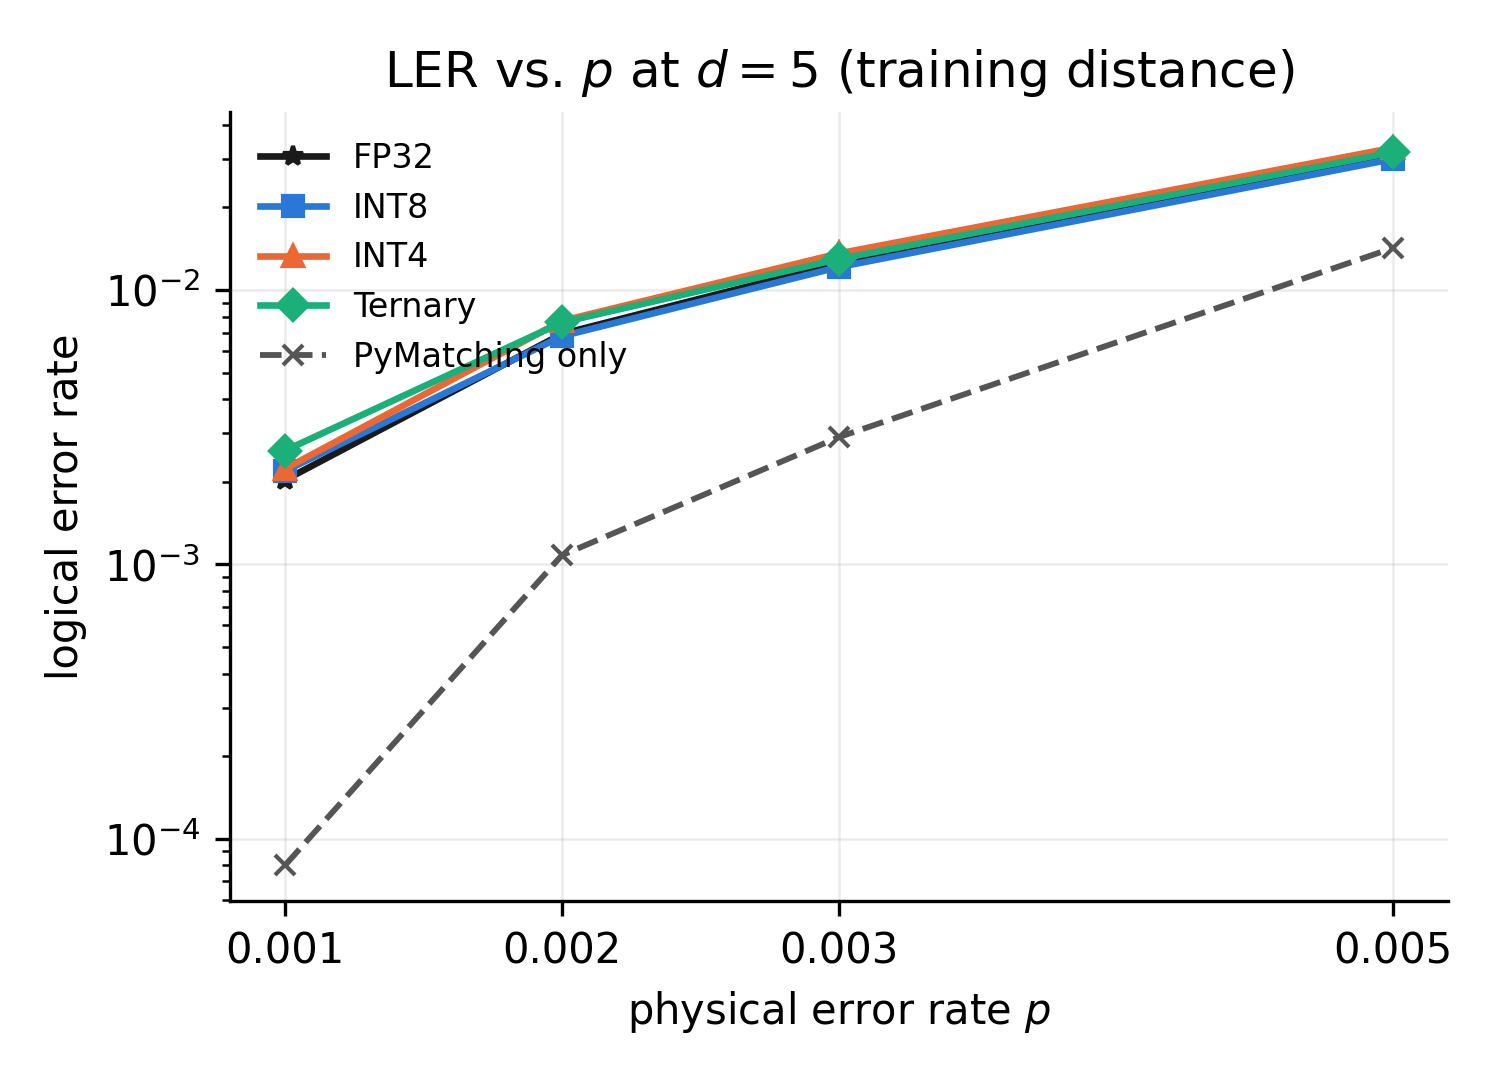
\includegraphics[width=\textwidth]{figures/fig1_ler_vs_p.png}
\caption{Logical error rate vs.\ physical error rate at \(d=5\) (the training distance). Every precision (FP32, INT8, INT4, ternary) sits above the PyMatching-only baseline across the full tested range.}\label{fig:ler-vs-p}
\end{figure}

\subsection{Distance generalization}\label{subsec:results-distance}
Figure~\ref{fig:ler-reduction} shows the LER reduction factor (baseline LER divided by pre-decoder LER; values below 1 indicate the pre-decoder made things worse) as a function of evaluation distance at the fixed operating point \(p=0.003\). At \(d=5\) this factor is already below 1 (\(\approx 0.23\) for FP32); by \(d=13\) it has fallen to \(\approx 2.4\times 10^{-4}\), roughly three further orders of magnitude worse. This is the opposite of the distance-generalization property a fully convolutional architecture is intended to provide, and is the central negative finding of this paper.

\begin{figure}[t]
\centering
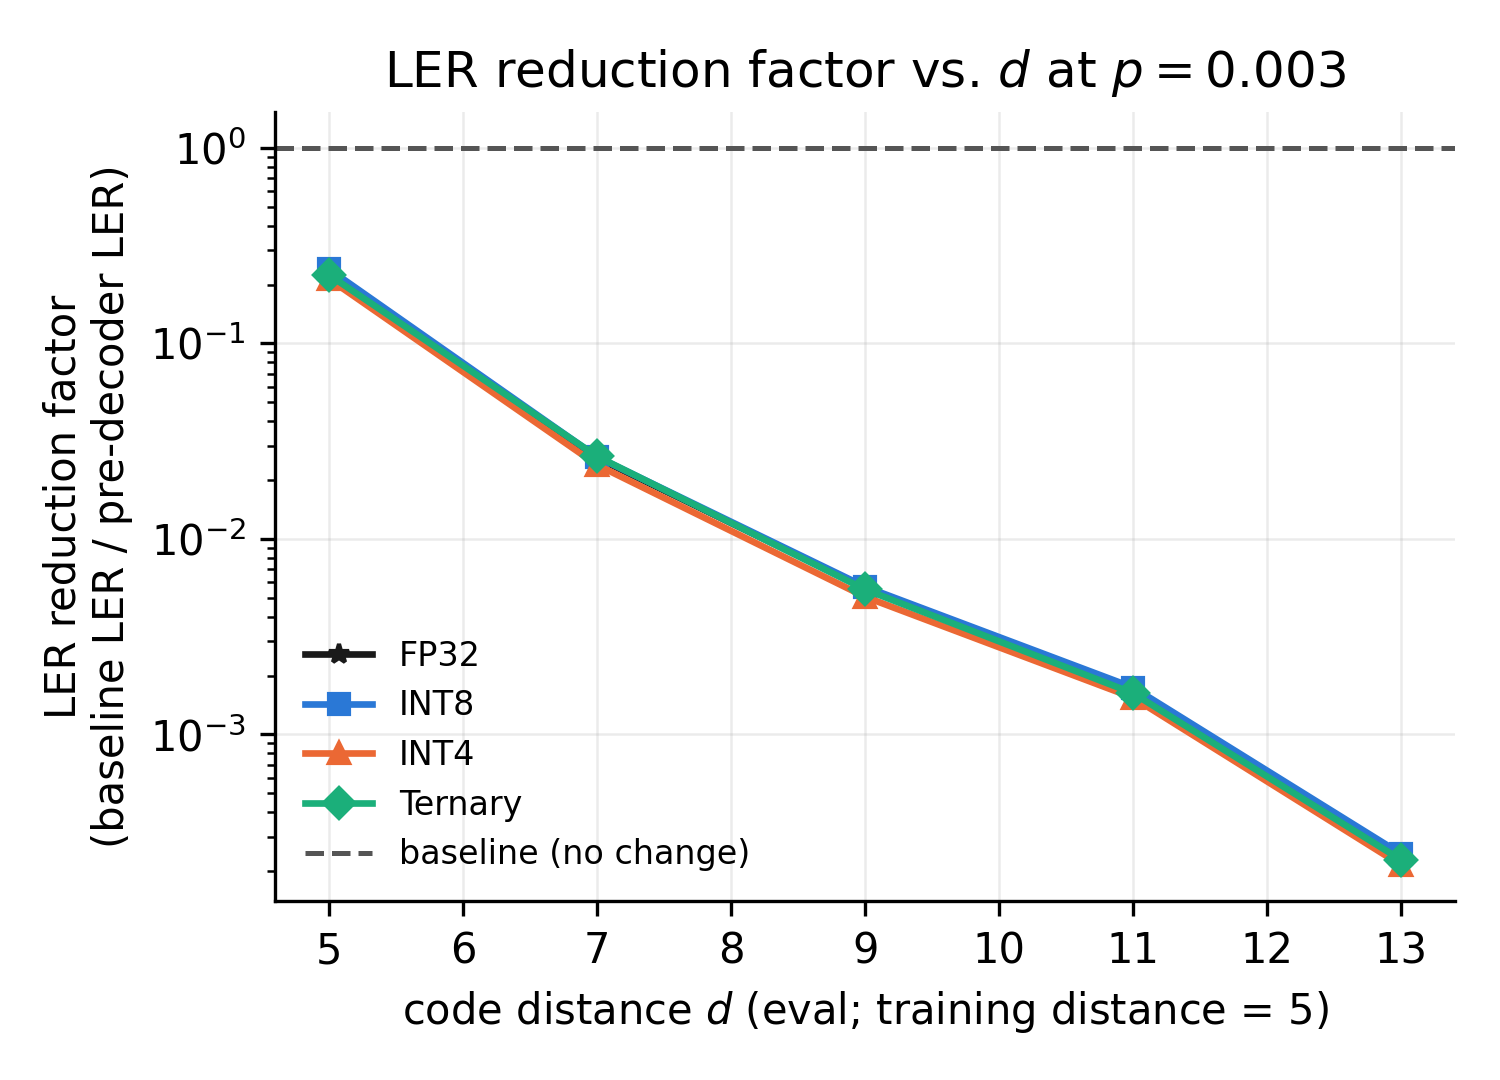
\includegraphics[width=\textwidth]{figures/fig2_ler_reduction_factor_vs_d.png}
\caption{LER reduction factor vs.\ evaluation distance at \(p=0.003\) (log scale). The dashed line at 1.0 marks "no change from baseline"; every curve is below it and falling.}\label{fig:ler-reduction}
\end{figure}

Syndrome density reduction, in contrast, remains substantial and roughly stable across the same distance range (Figure~\ref{fig:sdr}): 43--56\% of detection events are removed by the pre-decoder's correction at every tested distance. This is a genuinely different claim from LER improvement, and both are reported because they are both true: the pre-decoder is removing real detection events, but not accurately enough, and not in a way that the residual PyMatching decode benefits from.

\begin{figure}[t]
\centering
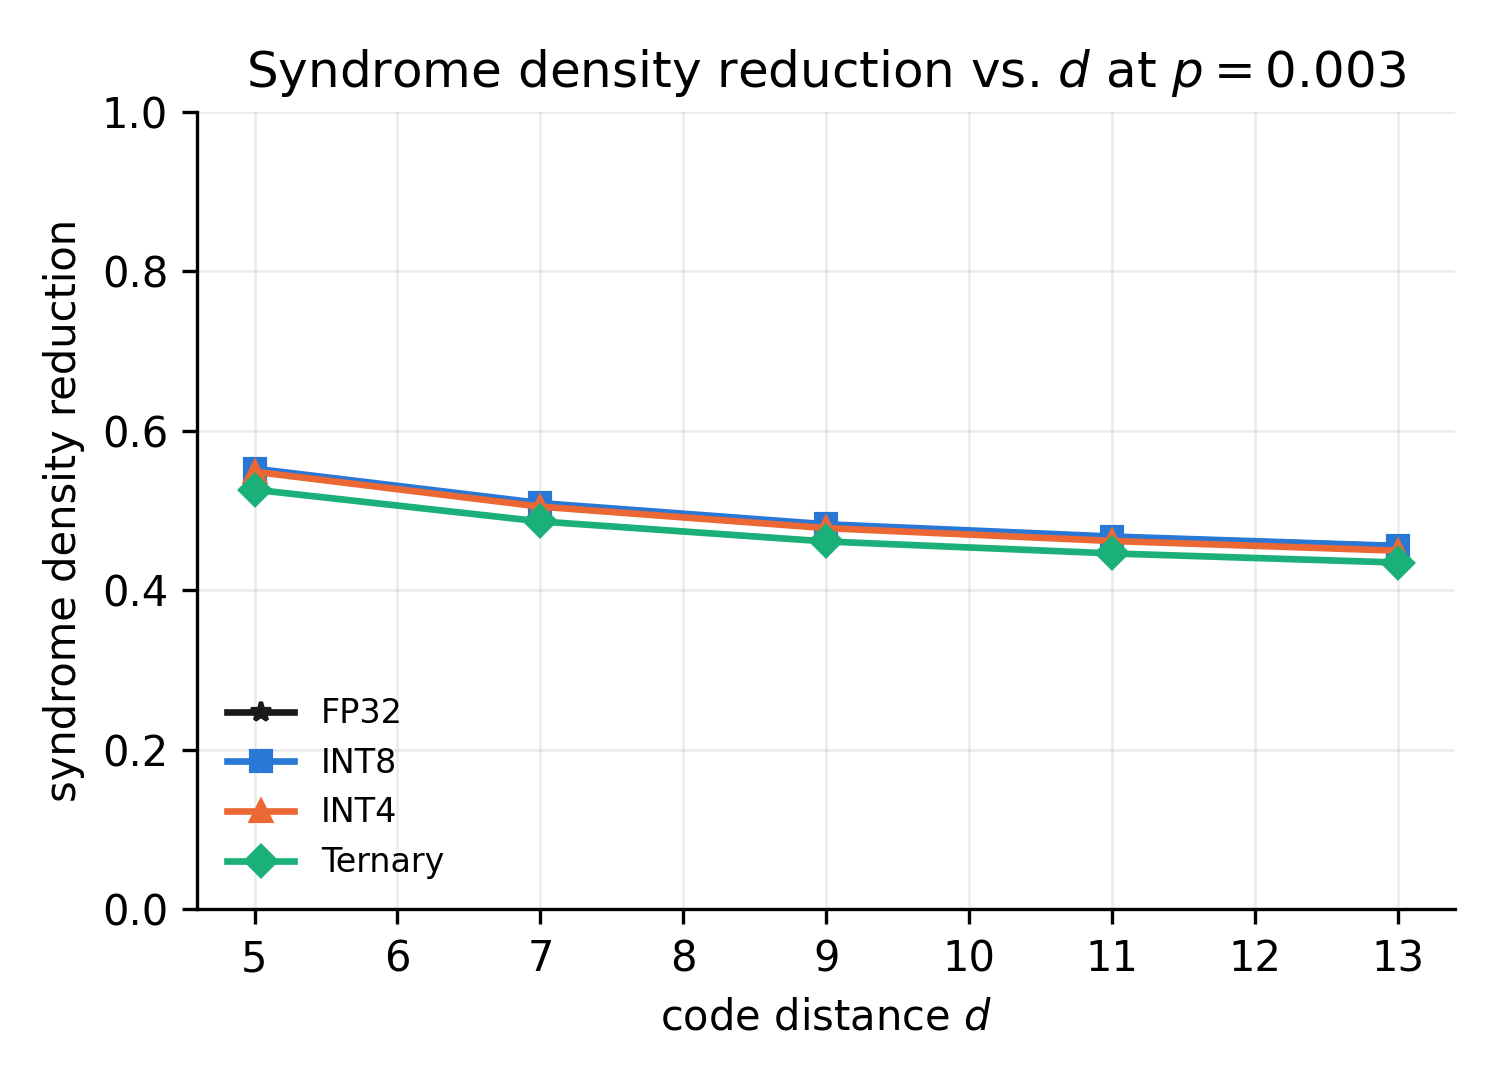
\includegraphics[width=\textwidth]{figures/fig3_sdr_vs_d.png}
\caption{Syndrome density reduction vs.\ distance at \(p=0.003\): stays real and substantial even as LER (Fig.~\ref{fig:ler-reduction}) does not improve.}\label{fig:sdr}
\end{figure}

\subsection{Quantization}\label{subsec:results-quant}
Table~\ref{tab:quant} reports the quantization sweep at \(d \in \{5,7\}\), \(p=0.003\) (the original Phase 3 sweep, used to export the fixed-point weights synthesized in Section~\ref{sec:hls}). INT8 and ternary track FP32 closely at both distances; INT4 shows a consistent regression of roughly 8--10\% relative LER. Figure~\ref{fig:pareto} shows the same comparison as an accuracy-vs-bit-width plot at \(d=5\).

\begin{table}[t]
\centering
\caption{Quantization sweep: logical error rate by precision and distance (\(p=0.003\), 100{,}000 shots).}\label{tab:quant}
\begin{tabular}{lrr}
\toprule
Precision & LER (\(d=5\)) & LER (\(d=7\)) \\
\midrule
FP32 & 0.01292 & 0.06593 \\
INT8 & 0.01258 & 0.06515 \\
INT4 & 0.01424 & 0.07124 \\
Ternary & 0.01303 & 0.06435 \\
\bottomrule
\end{tabular}
\end{table}

\begin{figure}[t]
\centering
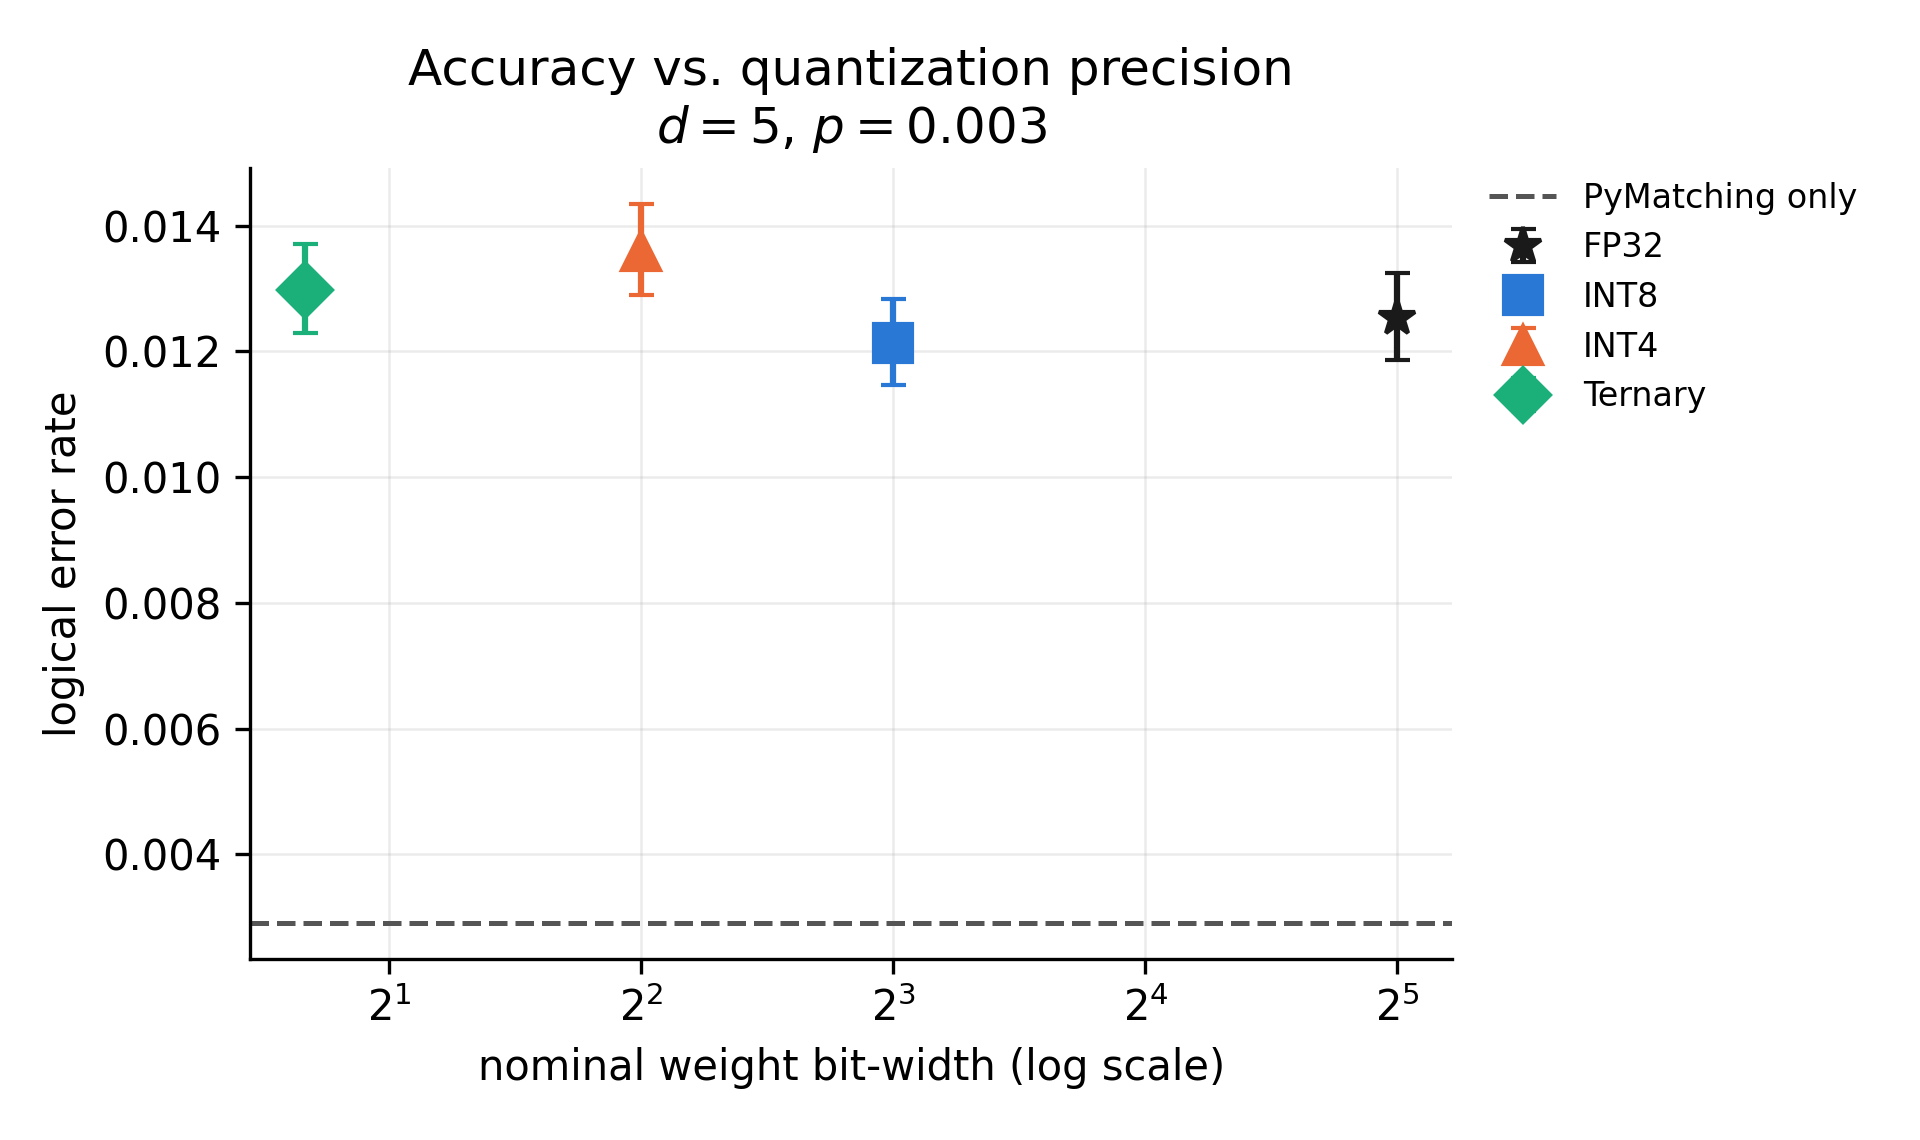
\includegraphics[width=\textwidth]{figures/fig6_pareto_precision.png}
\caption{Accuracy vs.\ nominal weight bit-width at \(d=5, p=0.003\) (log-scale x-axis; ternary plotted at \(\log_2 3\), its true information content). INT8 and ternary track FP32 closely; INT4 is the one consistent regression.}\label{fig:pareto}
\end{figure}

\subsection{HLS synthesis and the real hardware build}\label{subsec:results-hls-summary}
Results for the resource-explosion defect and its fix are reported in Table~\ref{tab:hls-before-after} (Section~\ref{subsec:results-hls}); the real, timing-closed build's numbers are reported in Table~\ref{tab:kernel-util-routed} and Section~\ref{subsec:results-hw}. Figure~\ref{fig:resources} visualizes the before/after device-wide utilization on a shared log axis, since the BRAM overshoot spans nearly three orders of magnitude and would otherwise dominate a linear-scale comparison.

\begin{figure}[t]
\centering
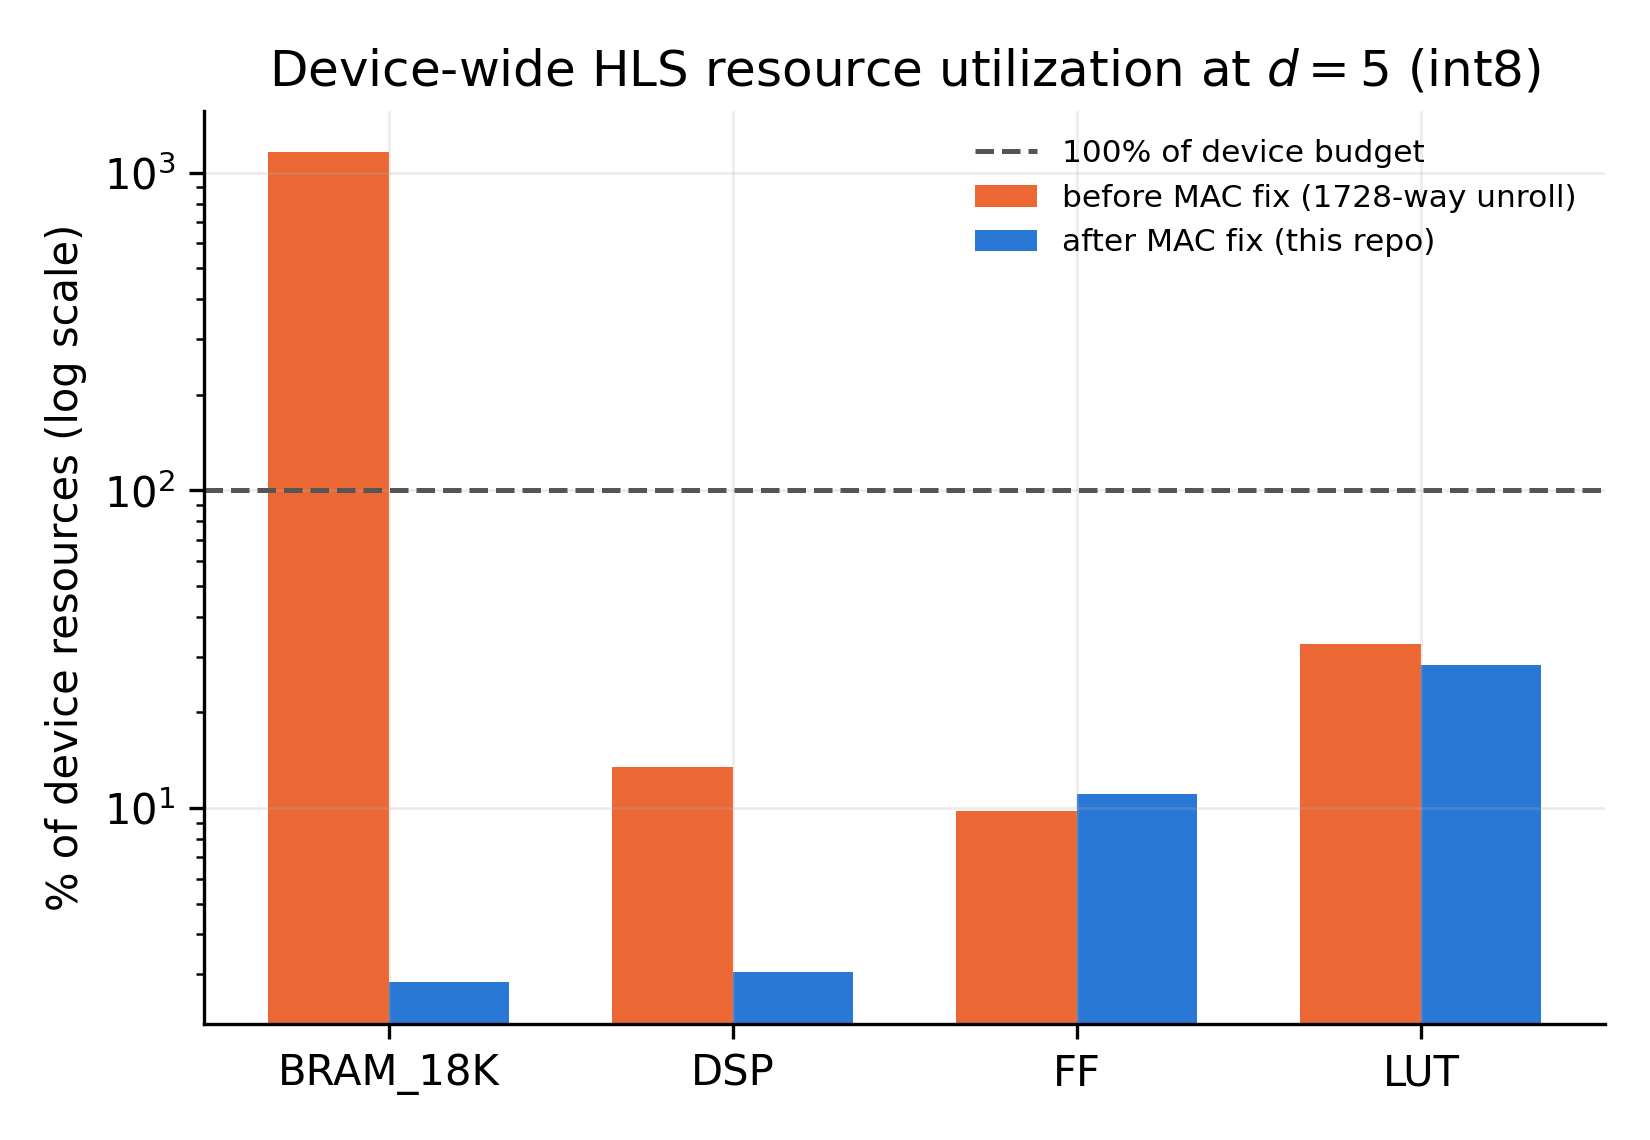
\includegraphics[width=\textwidth]{figures/fig5_resource_utilization_d5.png}
\caption{Device-wide HLS resource utilization at \(d=5\) (INT8), before and after the multiply-accumulate unroll fix. The dashed line marks 100\% of the device's resource budget.}\label{fig:resources}
\end{figure}

\subsection{Latency}\label{subsec:results-latency}
Figure~\ref{fig:latency} compares per-round latency across three real, measured pipelines: PyMatching alone (2.26\,\textmu s/round, CPU), the honest software-simulated pre-decoder-plus-PyMatching pipeline (43.8\,\textmu s/round, CPU, from the labeled-simulated fallback path), and the real, timing-closed FPGA kernel's own cycle count combined with the same CPU PyMatching decode time (3{,}056.9\,\textmu s/round; the FPGA kernel replaces only the pre-decoder stage, decode still runs on the host in this design).

\begin{figure}[t]
\centering
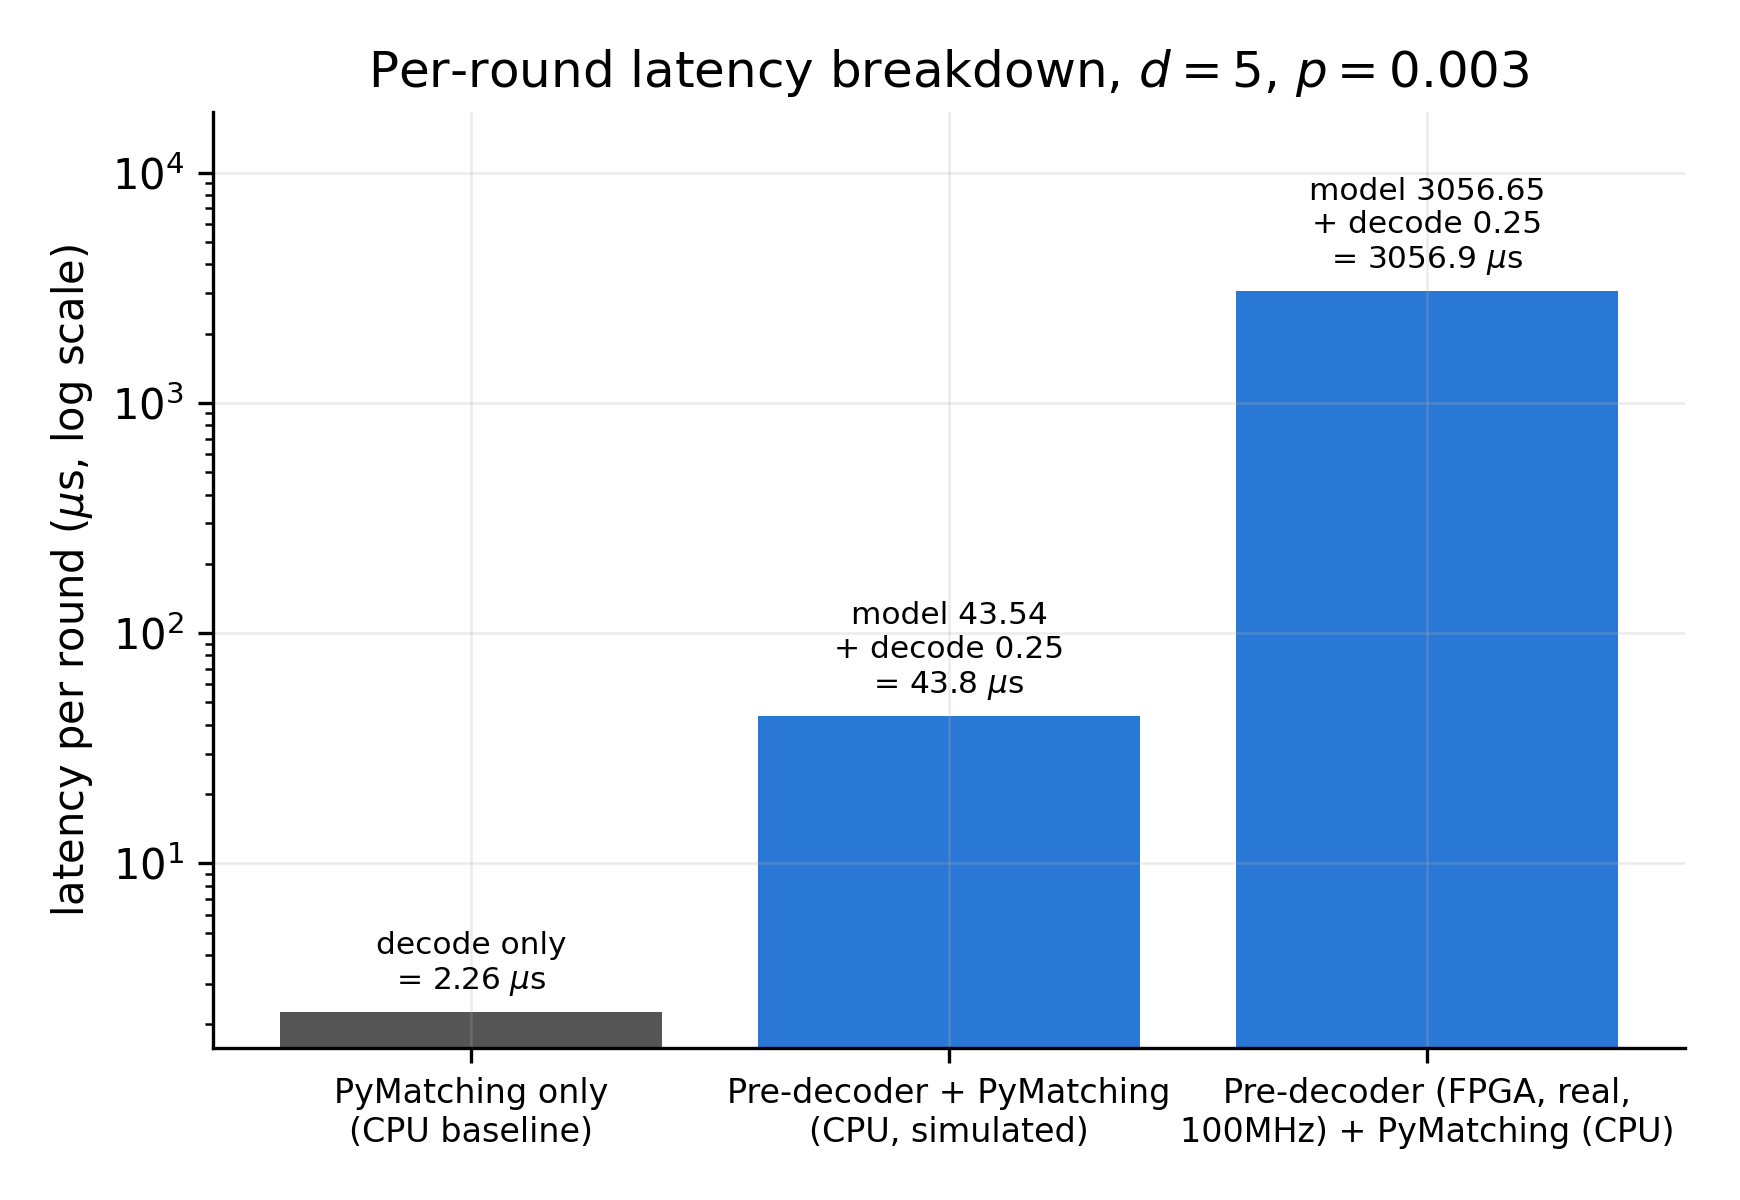
\includegraphics[width=\textwidth]{figures/fig4_latency_breakdown.png}
\caption{Per-round latency breakdown (log scale) across three real, measured pipelines at \(d=5, p=0.003\). Values are direct-labeled rather than area-stacked, since the decode segment (\(<\)2.3\,\textmu s in every bar) would otherwise be invisible against the much larger pre-decoder segment on a log axis.}\label{fig:latency}
\end{figure}

\section{Discussion}\label{sec:discussion}

\subsection{Why the pre-decoder underperforms and does not generalize}\label{subsec:discussion-why}
Several factors plausibly contribute to the gap between this reimplementation's result and the positive result the method is intended to provide, and this paper does not claim to have isolated a single root cause. The training budget used here (2M shots/epoch, 20 epochs, single CPU) is a deliberate, large reduction from the reference method's reported recipe (67M shots/epoch, 100 epochs, 8 GPUs) -- roughly a 1{,}600\(\times\) reduction in total training shots seen -- and undertraining is a plausible, likely major contributor on its own. The training target is also, by construction, a subset of the true error process: only DEM error mechanisms touching at most two detectors are included as positive training labels, leaving all higher-weight (3+ detector) events entirely unaddressed by the pre-decoder and left for PyMatching alone; this matches the method's own framing of removing "a large fraction," not all, of detection events, but bounds how much the pre-decoder could help even with perfect accuracy on its restricted target. Whether a longer training run, at the reference method's scale, would close some or all of this gap is a directly answerable empirical question that this project's CPU-only compute budget did not allow answering, and is the most important piece of follow-up work this paper identifies.

\subsection{The latency gap}\label{subsec:discussion-latency}
The measured real per-shot latency (13.0--15.3\,ms, Section~\ref{subsec:results-hw}) is approximately four orders of magnitude above the microsecond-scale target the method aspires to, and this gap is not primarily an artifact of clock frequency: even at the achievable \(\sim\)300\,MHz the unclosed-timing build ran at before its clock was lowered for closure, the cycle count itself (1{,}528{,}325 worst case) is the dominant factor, and that cycle count is a direct, load-bearing consequence of the same fix that resolved the BRAM overshoot (Section~\ref{subsec:results-hls}): de-unrolling the wide layer's input-channel reduction traded roughly a 64\(\times\) increase in that layer's cycle count for an 11\(\times\)-over-budget-to-2.8\%-of-budget reduction in BRAM usage. This is a real engineering tradeoff, not a bug: at the resource budget this design occupies now, there is substantial headroom (97\%+ of BRAM, 96\%+ of DSP) to spend on reclaiming throughput -- for example, a partial unroll wider than the current fully-serial reduction, or replicating the design to pipeline multiple shots concurrently -- that this paper did not attempt.

\subsection{What is, and is not, established by this work}\label{subsec:discussion-established}
It is established, with real measured evidence, that: quantization to INT8 or ternary costs negligible pre-decoder accuracy; the described neural architecture and correction scheme are numerically and architecturally sound in the sense that they synthesize correctly and match a bit-exact software model through RTL cosimulation; a real, resource-fitting, timing-closed bitstream for a kernel of this class can be built on the target hardware. It is not established that this specific, CPU-budget-constrained training run produces a pre-decoder that helps; the evidence available is that it does not, at the tested training budget and target distance, and that whatever benefit exists does not survive evaluation at larger distances.

\section{Conclusion}\label{sec:conclusion}

This paper described a complete, independent FPGA reimplementation of a neural pre-decoder for surface-code quantum error correction, evaluated honestly rather than selectively. The reimplementation surfaced and fixed several real, nameable defects along the way -- a receptive-field bug, a per-voxel correction design that actively harmed decoding, a silent bias-quantization error, a silent numeric-formatting bug that corrupted exported weight scales, two distinct HLS synthesis runaways, an 11\(\times\)-over-budget BRAM overshoot traced to a specific unrolled loop, and an unclosed timing-closure violation in the first successful place-and-route attempt -- and each is documented with the evidence that found it, not asserted. The headline accuracy result is negative at the tested training budget and target distance, and the paper reports that plainly rather than reframing around only the positive quantization and hardware-build results. Every number in this paper is generated by a committed, re-runnable script from committed data; the repository, including the exact commands used to reproduce every figure and table, is publicly available.

\backmatter

\section*{Acknowledgments}
This work is an independent reimplementation of a pre-decoder concept described by NVIDIA's \texttt{Ising-Decoding} work \cite{chamberland2026fast}; no source code, model weights, or other artifacts from that repository were used. The author thanks the maintainers of Stim \cite{gidney2021stim} and PyMatching \cite{higgott2022pymatching}, on which the simulation and baseline-decoding pipeline in this work directly depends.

\section*{Declarations}

\textbf{Funding:} This work received no external funding.

\textbf{Conflict of interest:} The author declares no conflict of interest.

\textbf{Data availability:} All code, synthesis reports, trained checkpoints' metrics, and figures are available at the public repository accompanying this paper.

\begin{thebibliography}{9}

\bibitem{fowler2012surface}
Fowler AG, Mariantoni M, Martinis JM, Cleland AN (2012) Surface codes: Towards practical large-scale quantum computation. Phys Rev A 86(3):032324

\bibitem{higgott2022pymatching}
Higgott O (2022) PyMatching: A Python package for decoding quantum codes with minimum-weight perfect matching. ACM Trans Quantum Comput 3(3):1--16

\bibitem{chamberland2026fast}
Chamberland C, et al (2026) Fast and accurate AI-based pre-decoders for surface codes. arXiv:2604.12841

\bibitem{gidney2021stim}
Gidney C (2021) Stim: a fast stabilizer circuit simulator. Quantum 5:497

\bibitem{das2022afs}
Das P, et al (2022) AFS: Accurate, fast, and scalable error-decoding for fault-tolerant quantum computers. In: Proc IEEE Int Symp High-Performance Computer Architecture (HPCA)

\bibitem{bengio2013ste}
Bengio Y, L\'{e}onard N, Courville A (2013) Estimating or propagating gradients through stochastic neurons for conditional computation. arXiv:1308.3432

\end{thebibliography}

\end{document}
